\documentclass[aspectratio=169, professionalfonts]{beamer}

\usepackage{mathtools} % \mathclap for shortening overbrace text

\usepackage{graphicx}
\usepackage{subfig}
\usepackage{longtable}
\usepackage{booktabs}
\usepackage{wrapfig}
\usepackage{rotating}
\usepackage[normalem]{ulem}
\usepackage{amsmath}
\usepackage{amssymb}
\usepackage{capt-of}

\usepackage{hyperref} \hypersetup{ colorlinks=true,
	linkcolor=blue, filecolor=magenta, urlcolor=cyan, pdftitle={Overleaf Example},
	pdfpagemode=FullScreen}

%% Personal macros across multiple projects
\input{components/combined-macros.tex}
%% Paper-specific macros

\usepackage[style=verbose,backend=biber, isbn=false, url=false, doi=false,
	eprint=false, dashed=false]{biblatex}
\addbibresource{my-biblatex-library.bib}

% Assumed directory structure is structure both VK and its associated files
% live in ./components/vk-theme
\usepackage{components/vk-theme/beamerthemeVK}

\author{John Sperger}
\date{March 8\textsuperscript{th} 2024}
\title{Value Function Inference}
\subtitle{A Moderately Technical Introduction}
\begin{document}
\maketitle

\section{Overview}
\begin{frame}{Outline}
	\tableofcontents[hideallsubsections]
\end{frame}
\begin{frame}[label={overview:objectives}]{Learning Objectives}
	We will cover: value function inference for a single-stage treatment policy /
	dynamic treatment regime (DTR)
	\vfill \pause
	At the end of today's talk you should be able to:
	\begin{itemize}
		\item Identify the fundamental challenge facing value function inference
		      that applies to all temporal settings.
		      \vfill \pause

		      %\item Provide an example of other problems in statistics that
		      %face a similar hurdle
		      %		\item Define the potential value function estimands and contrast the
		      %		      reasons for choosing them.

		\item Categorize the major approaches to inference in this setting

		      \vfill \pause

		\item Contrast the projection, bound, and bootstrap approaches to constructing confidence intervals
		      \vfill \pause

		\item Explain the connection between the finite-sample approach and the
		      asymptotic approaches
		      %\item Explain inference for OWL
		      %\item Name the keywords to search for to find relevant theory
	\end{itemize}
	\vfill
\end{frame}

% \begin{frame}{Key concepts}
%     Smoothness
%     \end{frame}

\subsection{Math notation}
\begin{frame}[label={sec:org00d2d44}]{Notation}

	Let $[K]$ denote the set $\{1, \ldots, K \}$ for a positive integer $K$. Assume
	the data is comprised of iid replicates:

	\begin{equation*}
		\left\{{\covarrv}_{\obsindex},\, {\armrv}_{\obsindex},\,
		{\resprv}_{\obsindex} \right\}_{\obsindex = 1}^{\maxobsindex}
	\end{equation*}

	%	following the standard convention where

	$\covarrv_{\obsindex} \in \covarspace \subseteq
		\symbb{R}^{\dimarmparam}$ denotes the covariates (contexts)

	$\armrv_{ \obsindex} \in \armspace$ denotes the treatment arm (arm,
	intervention, action), and

	$\resprv_{ \obsindex} \in \symbb{R}$ denotes the response (reward)

	\vfill \pause

	We'll use the potential outcome framework and denote the potential outcome 	$\po(\armobs)$

	\vfill \pause
	I'll use the index $\asymindex$ when discussing asymptotics and $\obsindex$ when discussing finite samples.	I'll try to maintain consistency but might slip up.
\end{frame}


\begin{frame}{Operator notation}
	\begin{itemize}
		\item $\covarrv_1, \ldots, \covarrv_{\maxobsindex}$ is an iid random sample from a
		      fixed but unknown distribution $\Pop$
		\item $\genericfun$ is a generic parametric function indexed by $\theta \in \Theta$
		\item $\hat{\theta} \in \Theta$ is a random variable constructed from the sample
		      $\covarrv_1, \ldots, \covarrv_{\asymindex}$
	\end{itemize}
	\vfill \pause

	$\Pop$ denotes the probability measure:
	\begin{equation*}
		\Pop \genericfun(\covarrv; \hat{\theta}) = \int \genericfun(\covarobs;\,\widehat{\theta}) \dv
		\Pop(\covarobs))
	\end{equation*}

	\vfill \pause $\Pn$ denotes the corresponding empirical measure:

	\begin{equation*}
		\Pn \genericfun(\covarrv; \hat{\theta}) = \asymindex^{-1}\sum_{i =
			1}^{\asymindex} \genericfun(\covarobs_{i};\,\hat{\theta})
	\end{equation*}
	\vfill \pause

	$\leadsto$ denotes convergence in distribution.

	\vfill
\end{frame}

\subsection{Treatment Policy Notation}

\begin{frame}{Treatment Policy Notation}
	A policy (aka DTR, treatment rule) $\pol$ is a function relating
	contexts and actions.

	\vfill
	Policies may be deterministic, $\pol: \covarspace
		\mapsto \armspace$ or stochastic
	$\pol: \covarspace \times \armspace \mapsto [0, 1]$.

	\vfill \pause

	Authors may write $\pol(\covarobs,
		\armobs)$, $\pol(\armobs \mid \covarobs)$, $\pol(\covarobs)$, or
	simply $\pol$ depending on what the author wishes to emphasize.

	\vfill \pause
	Define the value of a policy $\pol$ as
	\begin{equation*}
		\val(\pol) \doteq \E_{\covarrv}[\po(\armobs = \pol(\covarrv))]
		%	\polval = \val(\pol) \doteq \E_{\covarrv}[\po(\armobs =\pol(\covarrv))]
	\end{equation*}

	\vfill \pause
	An optimal policy $\optpol$ is any policy that satisfies
	\begin{equation*}
		\val(\optpol) \geq \val(\pol) \qquad \text{for all }\pol \in
		\polset
		% \polvalopt = \val(\optpol) \geq \val(\pol) \qquad \text{for all }\pol \in \polset
	\end{equation*}

	\vfill \pause
	Denote the estimated optimal policy $\polhatn$, and for conciseness, assume
	that there is a unique maximizer for every covariate value.

\end{frame}

\begin{frame}{Value Functions}
	Why don't I have Y here?
	\begin{enumerate}
		\item Conditional Value of the estimated optimal policy

		      $$\val(\polhatn) = \E_{\covarrv}[\polhatn(\covarrv) \vert \polhatn] = \Pop \polhatn(\covarrv)$$

		      \vfill \pause

		\item (Expected) Value of an estimated optimal policy
		      $$\E_{\covarrv}[\polhatn(\covarrv)]$$

		      \vfill \pause

		\item Value of the optimal policy (or, more broadly, any fixed policy)
		      $$\val(\optpol) = \E_{\covarrv}[\optpol(\covarrv)] = \Pop
			      \optpol(\covarrv)$$
	\end{enumerate}

	\vfill \pause
	These three will not generally be equivalent even asymptotically.
\end{frame}

\begin{frame}{Estimating the Value Function}
	There are two common approaches to estimating the value function:
	\begin{enumerate}
		\item Inverse Probability Weighting (IPW) / Importance Weighting

		\item Augmented Inverse Probability Weighting (AIPW) / Doubly Robust Estimation
	\end{enumerate}

\end{frame}
\begin{frame}{Other Distinctions}

	Let $\histpol(\armobs \mid \covarobs)$ denote the policy that was used to assign treatment
	during the experiment and $\pol(\armobs \mid \covarobs)$ the policy we are intersested in
	evaluating.

	\begin{columns}[T]
		\begin{column}{.5\textwidth}
			\ddef{Technical Word}{
				\begin{itemize}
					\setlength\itemsep{0.5em}
					\item[\textendash] On-policy $\pol = \histpol$
					\item[\textendash] Off-policy $\pol \neq \histpol$. Requires additional
						assumptions about the overlap between the policies, which
						may vary slightly but have the general flavor:

						$$\impwt =
							\frac{\pol(\covarobs)}{\histpol(\covarobs)}$$
				\end{itemize}
			}
		\end{column}
		\pause
		\begin{column}{.5\textwidth}
			\ddef{Technical Word}{
				\begin{itemize}
					\setlength\itemsep{0.5em}
					\item[\textendash] Data-derived or estimated policy
					\item[\textendash] Fixed policy

						\[\wmax \doteq \esssup_{\obsindex \in \NN, \armobs \in \armspace, \covarobs \in \covarspace} \frac{\pi(\armobs \mid \covarobs)}{h_{\obsindex}(\armobs \mid \covarobs)} \]
				\end{itemize}
			}
		\end{column}%
	\end{columns}


\end{frame}


% \begin{frame}{Today's Focus}
% 	Single-stage

% 	Fixed policy

% 	No parametric assumptions
% \end{frame}


\section{High-level Overview}
\begin{frame}{Nonregularity}
	Nonregular is the catch-all for when standard regularity conditions do
	not hold.
	\vfill \pause
	The general problem we'll be addressing is when the limiting
	distribution depends sharply on the parameter values.

	\vfill
	A common cause is a lack of
	\ddef{Smoothness}{
		A function $f$ is a smooth if it has continuous derivatives up to some
		desired order over some domain. The number of derivatives is problem-specific.
	}

	\vfill
	%	\tiny ``Continuously differentiable'' does not mean infinitely
	%	differentiable as a young me once confusedly thought.
\end{frame}

\begin{frame}{Examples of Nonregularity}
	Suppose $\covarrv_1, \ldots, \covarrv_{\asymindex}$ are iid copies of a random vector
	$\covarrv \in \mbbR^{p}$ drawn from an unknown distribution $P$. Let $\mu_0 = \Pop X
		= (\mu_{01}, \ldots, \mu_{0p})$

	\vfill \pause

	\textbf{Superefficient estimators}
	Define the estimator $\widetilde{\mu}_n$
	\begin{displaymath}
		\widetilde{\mu}_n = \begin{cases} \Pn X & \text { if } \Pn X \geq 1/4 \\
              0     & \text { if } \Pn X < 1/4\end{cases}
	\end{displaymath}

	\vfill \pause

	\textbf{Max of Means}
	Define $\theta_0$ as the component-wise maximum mean
	\begin{displaymath}
		\theta_0 = \maxsym_{j = 1}^p \mu_{0j} = \max_{j \in [p]} \mu_{0j}
	\end{displaymath}
\end{frame}

\begin{frame}{Is Nonregularity Avoidable?}

	``All \sout{happy families} regular estimators are alike; each \sout{unhappy
		family} nonregular estimator is unhappy in its own way.'' --- Markov,
	quoting Tolstoy\pause... possibly

	\vfill \pause
	For the superefficient estimator $\tilde{\mu}$ the form of the estimator, not
	the underlying estimand was the source of the nonregularity.

	\vfill \pause

	The nonregularity in value function inference is due to the nondifferentiability of the treatment
	policy/DTR, and this kind of nonregularity is unavoidable
	\footnote<4->{\fullcite{hirano2012Impossibility}}.
	\vfill
\end{frame}


\begin{frame}{PLACEHOLDER: Visual Examples of Approaches}
\end{frame}

\subsection{OWL}
\begin{frame}{OWL}
	\begin{figure}
		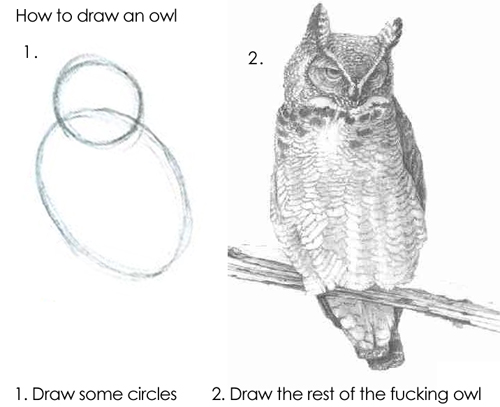
\includegraphics[width=.6\textwidth]{figures/how-to-draw-an-owl}
	\end{figure}
\end{frame}

\section{Detailed Overview}
\subsection{Max of Means Example}
\begin{frame}{Max of Means Limiting Distribution}

	Consider the estimators $\widehat{\mu}_{\asymindex} = \Pn \covarrv$  and $\widehat{\theta}_{\asymindex}$

	$$\widehat{\theta}_{\asymindex} = \maxsym_{j = 1}^p \widehat{\mu}_{\asymindex j}$$

	\begin{lemma}[Limiting Distribution of $\widehat{\theta}_{\asymindex} $]
		Define the set $\argmaxsetx{\mu_{0}} = \argmax_j \mu_{0j}$ and assume
		$\widehat{\mu}_n$ is regular $\rootn (\Pn - \Pop)X \convd \MVN(\zerovec, \Sigma)$. Then
		\begin{displaymath}
			\rootn (\widehat{\theta}_{\asymindex} - \theta_0) \convd \maxsym_{j \in \argmaxsetx{\mu_0}} Z_j
		\end{displaymath}
		where $Z \sim \MVN(\zerovec, \Sigma)$
	\end{lemma}

\end{frame}

\begin{frame}{Proof of the Limiting Distribution}
	Define the event $\eventn = \indfunx{\max_{k \notin \argmaxsetx{\mu_0}}
			\widehat{\mu}_{nk} \geq \max_{j \in\argmaxsetx{\mu_0}} \widehat{\mu}_{nj}}$. Note that
	\begin{enumerate}
		\item  $\eventn = \op{1}$
		\item When $E_n$ holds the maximizer(s) is not in $\argmaxsetx{\mu_0}$ and vice versa
		      %When $E_n$ holds the maximizer(s) is not in $\argmaxsetx{\mu_0}$
		      %    and the converse is true for the complement $E_n^{\text{C}} = 1 - E_n $
	\end{enumerate}

	\begin{align*}
		\rootn & (\widehat{\theta}_{\asymindex} - \theta_0) =  \maxsym_{j = 1}^p
		\rootn(  \widehat{\mu}_{\asymindex j} -
		\theta_0)                                                                      \\
		       & = (1 - \eventn + \eventn) \maxsym_{j \in\argmaxsetx{\mu_0}}^p \rootn(
		\widehat{\mu}_{\asymindex j} - \theta_0)                                       \\
		       & =  \maxsym_{j \in\argmaxsetx{\mu_0}}^p \rootn(
		\widehat{\mu}_{\asymindex j} - \theta_0) + \eventn \left(\maxsym_{k \notin\argmaxsetx{\mu_0}}^p \rootn(
		\widehat{\mu}_{\asymindex k} - \theta_0)  - \maxsym_{j \in\argmaxsetx{\mu_0}}^p \rootn(
		\widehat{\mu}_{\asymindex j} - \theta_0)\right)
	\end{align*}
\end{frame}

\begin{frame}{Proof Continued}
	{$${\color{red}\overbrace{\maxsym_{j \in\argmaxsetx{\mu_0}}^p \rootn(
				\widehat{\mu}_{\asymindex j} - \theta_0)}^{\mathclap{\substack{\text{{\small The
								desired }} \\ \text{{\small result}}}}}} + {\color{purple}\overbrace{\eventn \left(\maxsym_{k \notin\argmaxsetx{\mu_0}}^p \rootn(
				\widehat{\mu}_{\asymindex k} - \theta_0)  - \maxsym_{j \in\argmaxsetx{\mu_0}}^p \rootn(
				\widehat{\mu}_{\asymindex j} - \theta_0)\right)
			}^{\mathclap{\text{{\small A nuisance we'll show is $\op{1}$}}}}}$$} % see https://tex.stackexchange.com/questions/333744/a-more-beautiful-output-of-under-and-overbrace


\end{frame}

\begin{frame}{Visualizing the Problem --- Fixed $\delta$}
\end{frame}


\begin{frame}{Abstract problem}
	Nonsmooth functional of a smooth function

	Approach overview:

	$m$ out of $n$ directly approximate the nonsmooth functional - let the
	perturbations in $m_n$ be larger than the perturbations from the
	non-regularlity

	$m$ is $o(n)$ i.e. as $m \to \infty$ $\frac{m}{n} \to 0$
\end{frame}

\begin{frame}{Placeholder: Draw the approaches}
\end{frame}

\subsection{Asymptotic Aside}

\begin{frame}{What makes a good approximation?}
	Asymptotically valid does not guarantee a good approximation


	Uncertainty about the set of maximizers needs to be reflected in our
	approximation even if any positive difference results in asymptotic
	normality for $\widehat{\theta}_n$
\end{frame}

\subsection{Local Alternatives}
\begin{frame}{The Local Alternative}
	Idea: decompose into a static part and a part that changes with $n$

	$$\mu_n = \mu_0 + s h(n)$$

	$\mu_0, s \in \mbbR^{p)}$ are both fixed

	$h(n)$, often but not exclusively $n^{-1/2}$, controls the perturbations
\end{frame}



\begin{frame}{Construction a confidence interval}
\end{frame}

\begin{frame}{CI Proof}
\end{frame}



\section{Constructing Asymptotic Confidence Intervals}
\subsection{Regularization}
\begin{frame}{Asymptotic Approach Overview}

	% Please add the following required packages to your document preamble:
	% \usepackage{booktabs}
	\begin{table}[]
		\begin{tabular}{@{}lcccc@{}}
			\toprule
			                   & \begin{tabular}[c]{@{}c@{}}Theoretical \\ Guarantees\end{tabular}
			                   & \begin{tabular}[c]{@{}c@{}}Easy to \\ Implement\end{tabular}
			                   & Conservative
			                   & \begin{tabular}[c]{@{}c@{}}Empirical \\ Performance\end{tabular}                                                           \\
			\midrule
			Projection sets    & $\checkmark^{+}$                                                  & \symbol{"2610}   & $\checkmark^{+}$ & $\checkmark$     \\
			Bounding           & $\checkmark^{+}$                                                  & \symbol{"2610}   & $\checkmark$     & \checkmark       \\
			\mon  \, Bootstrap & $\checkmark$                                                      & $\checkmark^{+}$ & \symbol{"2610}   & \checkmark       \\
			Regularization     & \symbol{"2610}                                                    & $\checkmark$     & \symbol{"2610}   & $\checkmark^{+}$ \\
			\bottomrule
		\end{tabular}
	\end{table}

	\vfill \pause
	Regularization may induce infinite bias in certain scenarios.
\end{frame}

\begin{frame}{Not recommended: (Current) Regularization Approaches}
\end{frame}
\subsection{Projections}
\begin{frame}{Projection Region Big Picture}
	%	Recall our formulation $\theta_n = \theta_0 + h(n)s$
	\begin{itemize}
		\item The empirical estimator $\widehat{\mu}_n = \Pn X$ is well-behaved (regular, asymptotically normal)
		      \vfill \pause
		\item If we knew $\mu_0$ forming confidence intervals for ${\theta}_0$
		      would be simple --- we'd know $\mu_{01}$ is the maximizer and
		      construct a CI for $\mu_{01}$
	\end{itemize}
	\vfill \pause
	Solution:
	\begin{enumerate}
		\item Determine all plausible values of $\mu_0$ using the $(1- \alpha)$ CI
		\item For each plausible value of $\mu_0$, construct a CI for ${\theta}_0$
		      treating the plausible $\mu_0$ as fixed
		\item Take a union over over all of these CIs
	\end{enumerate}
	\vfill \pause
	Can be very conservative

	%	Particularly in the context of DTRs because
\end{frame}
\begin{frame}{Projection Confidence Set}
	Let $\waldset$ denote a $(1-\alpha)$ confidence set $\mu_0$. For concreteness, take
	the Wald CI

	$$\waldset = \waldsetdef$$

	\vfill \pause
	\ddef{Projection Confidence Set}{
		\begin{displaymath}
			\projset = \projsetdef
		\end{displaymath}
		is a valid confidence interval for $\theta_0$
	}
\end{frame}
\begin{frame}{Projection Proof}
\end{frame}

\begin{frame}{Adaptive Projection Regions}
\end{frame}
\begin{frame}{Fundamental Ideas}
\end{frame}
\begin{frame}{Fundamental Math}
\end{frame}
\begin{frame}{Practical Improvements}
	Double bootstrap
\end{frame}



\subsection{Adaptive CIs by Bounding}
\begin{frame}{Bound-based}
\end{frame}
\begin{frame}{Fundamental Ideas}
\end{frame}
\begin{frame}{Fundamental Math}
\end{frame}
\begin{frame}{Practical Improvements}
	Double bootstrap
\end{frame}

\subsection{\mon Bootstrap}
\begin{frame}{The $m$-out-of-$n$ Bootstrap}
\end{frame}
\begin{frame}{Fundamental Ideas}

	Caveat: Not as straightforwardly valid as Projection and Bounding approaches
	(modulo a certain definition of ``straightforward''), and can fail
	\autocite{andrews2010Asymptotic}
\end{frame}
\begin{frame}{Practical Improvements}
	Double bootstrap
\end{frame}


\section{Value Function Inference}
\begin{frame}{Setup}
	\begin{itemize}
		\item	Two arms $\armrv \in \{-1, 1\}$
		\item $\polhatnx = \sign(\covarobs^{\trans}\widehat{\beta}_{\asymindex})$
	\end{itemize}

	\begin{displaymath}
		\nonregindclass = \nonregindclassdef
	\end{displaymath}
\end{frame}

\begin{frame}{Assumptions}
\end{frame}

\begin{frame}{Joint Distribution Before Maximizing}

	\begin{displaymath}
		\rootn \begin{bmatrix}\Pn - Pop_{\asymindex} \\
			\betahatn - \betao     \\
			(\Pn - \Pop_{\asymindex})\resprv \indfunx{\armrv \covarrv^{\trans}\betao
				> 0}\end{bmatrix} \convd \begin{pmatrix} \mbbT \\ \mbbZ \\
			\mbbW\end{pmatrix}
	\end{displaymath}

	where

	\begin{itemize}
		\item $\mbbT$ is a Brownian Bridge indexed by $\mbbR^p$
		\item $\mbbZ$ and $\mbbW$ are normal
	\end{itemize}
\end{frame}

\begin{frame}{Distribution after Maximizing}
	\begin{displaymath}
		\rootn (\valhatn (\betahatn) - \val(\betahatn)) \convd \mbbT(\mbbZ + s)
		+ \mbbW
	\end{displaymath}

	where $s$ is a local parameter

\end{frame}

\begin{frame}{Life at the Boundary}
	The boundary is the source of the action

	In finite samples we can't identify observations that, in expectation, are
	near the boundary vs. on the boundary.

	This shows up in many proofs. Use the good old multiply by one trick using
	indicators for being on/not on the boundary.

\end{frame}

\section{Avoiding Nonregularity}
\begin{frame}{Alternatives to Asymptotics}
	If the blow-up happens in the limit, what if we just don't take it to the limit?
\end{frame}

\begin{frame}{Finite-sample bounds}
	Similar in spirit to the asymptotic bound-based approach, but with Martingales
	playing the role of the nicely behaved functions.

	More specifically test super-martingales. Recall that a super martingale is
	a stochastic process satisfying

	$$\E[Z(\obsindex + s) | Z(\obsindex)] \leq Z(s) \forall \obsindex, s \in \mbbN^+$$

	A test super-martingale $M_t$ is a non-negative super-martingale that under
	the null $\E_{P_0}[M_\obsindex] \leq 1$ at any time $\obsindex$
\end{frame}

\begin{frame}{Additional Notation of Note}
	Let $\histobs_{\obsindex}(\armrv_{\obsindex}, \covarrv_{\obsindex}) =
		\prob(\armrv_{\obsindex} = \armobs \mid \covarrv_{\obsindex} = \covarobs, \histspace_{t-1})$

	\[\impwtt \doteq \impwtdef \]
\end{frame}

\begin{frame}{Assumptions in this Setting}
	$\resprv$ is bounded, and for convenience we'll assume $\resprv \in [0,1]$

	$\polval_{\obsindex} \doteq \E_{\pol} [\resprv_{\obsindex} \mid \history_{\obsindex-1}]$
	Adapted

	Exogenous

	$$\prob(\armrv_{\obsindex} \mid \histspace_{\obsindex - 1}) =
		\prob(\armrv_{\obsindex} \mid \covarrv_{\obsindex})$$

	Common assumption on importance weights

	\[\wmax \doteq \esssup_{\obsindex \in \NN, \armobs \in \armspace, \covarobs \in
			\covarspace} \frac{\pi(\armobs \mid \covarobs)}{h_{\obsindex}(\armobs \mid
			\covarobs)} \] is finite.
\end{frame}

\begin{frame}{Assumptions for the method}
\end{frame}

\begin{frame}{Confidence Sequences}
	\begin{definition}[Confidence Sequence]
		We say that a sequence of intervals $[L_\obsindex, U_\obsindex]_{\obsindex=1}^\infty$ is a confidence sequence for the parameter $\theta \in \RR$ if
		\begin{equation*}\label{eq:cs}
			\prob \left ( \forall \obsindex \in \NN,\ \theta \in [L_\obsindex, U_\obsindex] \right ) \geq 1-\alpha \end{equation*}
		or equivalently,
		\begin{equation*}
			\prob \left ( \exists \obsindex \in \NN : \theta \notin [L_\obsindex, U_\obsindex] \right ) \leq \alpha
		\end{equation*}
	\end{definition}

	\vfill \pause
	For comparison, recall that a $(1- \alpha)$ confidence interval (CI) satisfies

	$$\forall \obsindex \in \NN,\ \prob(\theta \in [L_\obsindex, U_\obsindex]) \geq 1-\alpha$$
\end{frame}

\begin{frame}{Key Result}
	Define the weighted rewards $\phi_\obsindex^\IWL \doteq \impwtt \resprv_\obsindex$ and $\phi_\obsindex^\IWU \doteq
		\impwtt(1-\resprv_\obsindex)$
	\vfill
	Let   $(\lambda_t^L(\candpolval))_{t=1}^\infty$ be any $[0, 1/\candpolval)$-valued
	predictable sequence

	\vfill
	\begin{equation}\label{eq:kmr-cs}
		L_t^\IW \doteq \inf\left \{ \candpolval \in [0, 1] : \prod_{i=1}^t \left ( 1 + \lambda_i^L(\candpolval) \cdot (\phi_t^\IWL - \candpolval) \right ) < \frac{1}{\alpha} \right \}
	\end{equation}
	forms a lower $(1-\alpha)$ confidence sequence for $\polval$, meaning
	\vfill                  \vfill
	$\prob(\forall t \in \NN,\ \polval \geq L_t^\IW) \geq 1-\alpha$.
\end{frame}

\begin{frame}{Practical Improvements}
	\begin{itemize}
		\item Double robustness
		\item Trimming the observed rewards
		\item Empirical weights
	\end{itemize}
\end{frame}

\begin{frame}{From Sequence to Interval}
	Suppose that all we care about is a $(1 - \alpha)$ CI after $\maxobsindex$
	observations.

	\vfill
	A CS is also trivially a CI at a fixed time, but the width of the interval
	will be wider than if we only needed to guarantee coverage at one point in
	time.

	\vfill \pause

	\begin{lemma}[The minimum and maximum bounds of a $1 - \alpha$ confidence
			sequence form a $1 - \alpha$ confidence interval.] Define lower and upper bounds, $L^{\text{CI}}$ and
		$L^{\text{CI}}$, as
		$$L^{\text{CI}} = \max_{\obsindex \leq \maxobsindex}
			L_{\obsindex}^{\text{CS}} \qquad \text{ and } U^{\text{CI}} = \max_{\obsindex \leq
				\maxobsindex} U_{\obsindex}^{\text{CS}}$$

		Then $(L^{\text{CI}},\, U^{\text{CI}})$ is a $(1 - \alpha)$ confidence
		interval for $\val(\pol)$
	\end{lemma}
\end{frame}

\begin{frame}{What we didn't get to}
	Comparing multiple policies

	Off policy evaluation
\end{frame}
\section{Where Next?}

\begin{frame}{Where to Start}
	\vfill

	Start with Chapter 10 of \cite{tsiatis2019Dynamic}
	\vfill

\end{frame}

\begin{frame}{General Theory -- Asymptotic}
	\vfill
	\begin{itemize}
		\item Chapter 3 of \cite{tsiatis2006Semiparametric}
		      \vfill
		\item Chapters 6 and 7 of \cite{vandervaart2000Asymptotic}
		      \vfill
		\item \cite{kosorok2008Introduction}
		      \vfill
		\item Important Paper: \cite{hirano2012Impossibility}
		      \vfill


		\item 	\cite{bibaut2021PostContextualBandit}
		      \vfill
	\end{itemize}
\end{frame}

\begin{frame}{Precision Medicine}
	\vfill
	\begin{itemize}
		\item \cite{laber2014Dynamic}
		      \vfill

		\item 	\cite{luedtke2016Statistical}
		      \vfill

		\item 	\cite{shi2022Statistical}

		\item \cite{hadad2021Confidence}
	\end{itemize}
	\vfill

\end{frame}

\begin{frame}{General Theory -- Non-asymptotic}
	\vfill
	\begin{itemize}
		\item \cite{waudby-smith2022Anytimevalid}
		      \vfill

		      \item\cite{howard2021Timeuniform}
	\end{itemize}
	\vfill

	\begin{frame}{Conformal Inference?}
		Stuff that might be relevant but I haven't looked into it yet.
		Prediction intervals not CIs. More cites because this list isn't
		as filtered.
		\begin{itemize}
			\item \fullcite{vovk2009OnLine}
			      \vfill
			\item \fullcite{chernozhukov2018Exact}
			      \vfill
			\item \fullcite{barber2021Predictive}
			      \vfill
			\item \fullcite{lei2021Conformal}
			      \vfill
			\item \fullcite{jin2023Sensitivity}
			      \vfill
		\end{itemize}
	\end{frame}

\end{frame}

\appendix
\printbibliography

\end{document}
%%% Local Variables:
%%% mode: LaTeX
%%% TeX-master: t
%%% End:
